% E-06 paper section stub (Engineering, 2026-11-23). Not yet in paper/; HQ decides placement.
% Needs: booktabs, graphicx; the paper's macros (\btheta, \bD, \rhotau). Figure/table files: figs/fig_e06_headline_rough.pdf,
% tables/e06_main_table_rough.tex (full-radius and diagnostics tables for the supplement: tables/e06_main_table.tex,
% tables/e06_supp_table.tex, tables/e06_supp_diagnostics.tex). Numbers: tables/e06_slopes_all.csv (8400 fits, NOTS job 2858783).

\subsection{Empirical contraction rates}
\label{sec:sim:rates}

We check the contraction rates of Section~\ref{sec:theory} directly. As in the large-prior literature, we regress the log of the contraction radius on $\log n$ and compare the slope with the proved exponent.

\paragraph{Design.}
\begin{itemize}
 \item \emph{Data.} Two truths at $u_i=i/n$: a $C^1$ piecewise quadratic with three kinks (finite $V$) and $\sin(2\pi u)$. Five noise laws: Gaussian, Laplace, $t_3$, $t_2$ and Cauchy, all scaled to the same density at the median, so that they differ only in their tails. Two levels, $\tau\in\{0.5,0.9\}$.
 \item \emph{Sizes and seeds.} $n=1000,2000,\ldots,32000$ and $20$ seeds; a seed fixes the data across $n$ and across the arms below.
 \item \emph{Penalty schedules.} The penalty $\lambda\sigma$ follows $c\,n^{a}$ for the primary schedule $\lambda_n\propto n^{5/2}/V$ ($a=5/2$, predicted slope $-5/6$), the fallback $\lambda_n\propto(n^3/V)^{3/4}$ ($a=9/4$, $-3/4$), and the tuning of \citet{madrid2022risk} ($a=15/7$, $-5/7$).
 \item \emph{Calibration.} The constant $c$ is calibrated once per truth, noise law and $\tau$ at $n_0=500$, by minimising the risk of the posterior mode. The constant is capped so that every cell stays in the many-mode regime $n\lambda^{-1/3}\ge 10$; the cap binds for three of the twenty calibrations.
 \item \emph{Scale.} Two values of $\sigma$: $1.1\,\bar\sigma$ with $\bar\sigma=\tau(1-\tau)/f(q_\tau)$, inside the theorem, and the paper's pseudo-true scale $\sigma_0=\E\rhotau(\varepsilon-q_\tau)$, which lies below $\bar\sigma$ for every law except Laplace and $t_2$ at $\tau=\tfrac12$.
 \item \emph{Sampler and measure.} Each posterior is sampled exactly by a banded Gibbs sampler with $\lambda$ and $\sigma$ fixed. The contraction radius $\hat q_n$ is the $95\%$ posterior quantile of $\Delta^2_n(\btheta-\btheta^*)$. We fit the slope of the seed-median $\log\hat q_n$ on $\log n$ by least squares, with a $95\%$ paired bootstrap interval over seeds.
\end{itemize}

\paragraph{The rough component.}
The theorem bounds the full $\Delta_n^2$. Its three unpenalised (quadratic) directions add a parametric term of order $3/(n\kappa)$, $\kappa=f(q_\tau)/\sigma$, which is comparable to the $n^{-5/6}$ rough term for $n\le 32{,}000$ and pulls the fitted slope toward $-1$. We therefore report the radius $\hat q_n^{\perp}$ of the rough component $P^{\perp}(\btheta-\btheta^*)$, with the quadratic fit removed, in the main text, and the full radius in Supplement~\ref{app:sim:rates}; both are consistent with the theory.

\paragraph{Results.}
\begin{itemize}
 \item \emph{Headline cell.} Figure~\ref{fig:rates} shows the three schedules for the piecewise-quadratic truth with Gaussian noise, $\tau=\tfrac12$ and $\sigma=1.1\bar\sigma$. The fitted slopes are $-0.84$ $[-0.86,-0.83]$ for the primary schedule (theory $-5/6$), $-0.77$ $[-0.78,-0.75]$ for the fallback ($-3/4$) and $-0.74$ $[-0.75,-0.72]$ for the tuning of \citet{madrid2022risk} ($-5/7$). The order matches the theory.
 \item \emph{Primary schedule, all configurations.} Table~\ref{tab:rates} reports the primary schedule across noise laws, levels, truths and both scales. The slopes lie between $-0.80$ and $-0.89$, and the interval contains $-5/6$ in $33$ of the $40$ configurations; the exceptions are slightly steeper, at $\tau=\tfrac12$.
 \item \emph{Fallback and Madrid Padilla--Chatterjee schedules.} These are $0.02$ to $0.06$ steeper than their exponents. This is a finite-$n$ effect: at these sample sizes the local exponent of the posterior spread in $\log\lambda$ is about $-0.36$ rather than its asymptotic $-1/3$, so the slope along $\lambda\propto n^{a}$ is about $-0.36\,a$.
 \item \emph{Contraction probability.} The posterior probability of the ball of twice the predicted radius, $\Pi(\Delta_n^2>2\varepsilon_n^2\mid y)$ with $\varepsilon_n^2\propto n^{-5/6}$, never exceeds $0.014$ and decreases with $n$.
 \item \emph{The paper's scale $\sigma_0$.} The $\sigma_0$ arm gives the same slopes as $1.1\bar\sigma$ (median difference $-0.008$), even though it lies outside the proved range for most laws, including the heavy-tailed $t_2$ and Cauchy. This is consistent with the sandwich comparison of the rough component, which shows no variance inflation below $\bar\sigma$. It is empirical support beyond the proved range, not a theorem.
\end{itemize}

\begin{figure}[t]
 \centering
 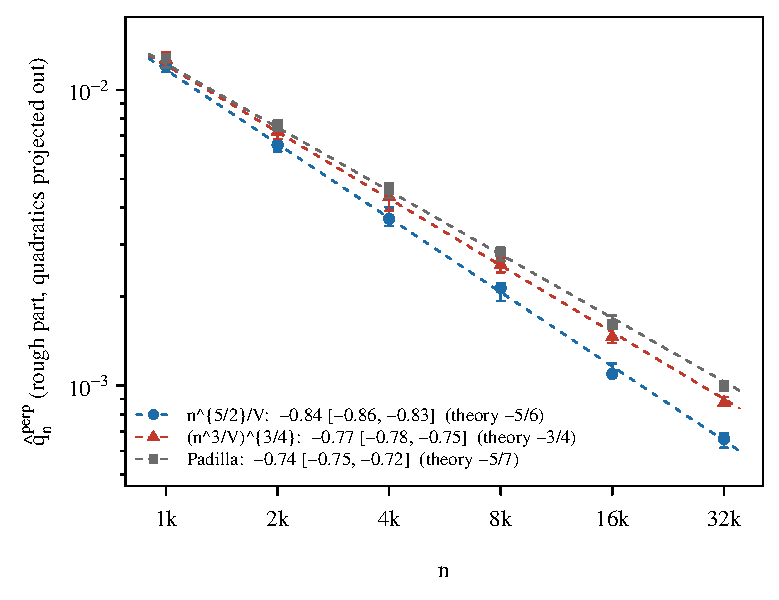
\includegraphics[width=0.62\textwidth]{figs/fig_e06_headline_rough.pdf}
 \caption{Contraction radius of the rough component against $n$ (log scales), for the piecewise-quadratic truth with Gaussian noise, $\tau=\tfrac12$ and $\sigma=1.1\bar\sigma$. Points are seed medians, with $95\%$ bootstrap intervals over $20$ seeds; dashed lines have the theoretical slopes. The legend gives each fitted slope and its interval.}
 \label{fig:rates}
\end{figure}

\begin{table}[t]
 \centering
 \caption{Fitted slope of $\log\hat q_n^{\perp}$ on $\log n$ under the primary schedule $\lambda_n\propto n^{5/2}/V$ (theory $-5/6\approx-0.833$), with $95\%$ paired bootstrap intervals; $n=1000$--$32000$, $20$ seeds per cell. Noise laws share the density at the median. The full-radius table, the other schedules and per-cell diagnostics are in Supplement~\ref{app:sim:rates}.}
 \label{tab:rates}
 \small
 \begin{tabular}{llcccc}
\toprule
 & & \multicolumn{2}{c}{piecewise quadratic} & \multicolumn{2}{c}{sine} \\
\cmidrule(lr){3-4}\cmidrule(lr){5-6}
noise & $\tau$ & $\sigma = 1.1\bar\sigma$ & $\sigma = \sigma_0$ & $\sigma = 1.1\bar\sigma$ & $\sigma = \sigma_0$ \\
\midrule
Gaussian & 0.5 & $-0.84$ {\scriptsize $[-0.86, -0.83]$} & $-0.84$ {\scriptsize $[-0.87, -0.81]$} & $-0.84$ {\scriptsize $[-0.85, -0.83]$} & $-0.85$ {\scriptsize $[-0.87, -0.81]$} \\
 & 0.9 & $-0.82$ {\scriptsize $[-0.86, -0.79]$} & $-0.81$ {\scriptsize $[-0.88, -0.73]$} & $-0.83$ {\scriptsize $[-0.87, -0.81]$} & $-0.80$ {\scriptsize $[-0.89, -0.76]$} \\
Laplace & 0.5 & $-0.88$ {\scriptsize $[-0.90, -0.86]$} & $-0.88$ {\scriptsize $[-0.90, -0.86]$} & $-0.88$ {\scriptsize $[-0.89, -0.85]$} & $-0.89$ {\scriptsize $[-0.90, -0.85]$} \\
 & 0.9 & $-0.81$ {\scriptsize $[-0.85, -0.78]$} & $-0.82$ {\scriptsize $[-0.88, -0.72]$} & $-0.84$ {\scriptsize $[-0.87, -0.82]$} & $-0.80$ {\scriptsize $[-0.90, -0.76]$} \\
$t_3$ & 0.5 & $-0.85$ {\scriptsize $[-0.86, -0.82]$} & $-0.85$ {\scriptsize $[-0.87, -0.82]$} & $-0.85$ {\scriptsize $[-0.87, -0.83]$} & $-0.85$ {\scriptsize $[-0.86, -0.82]$} \\
 & 0.9 & $-0.83$ {\scriptsize $[-0.86, -0.80]$} & $-0.81$ {\scriptsize $[-0.90, -0.73]$} & $-0.85$ {\scriptsize $[-0.88, -0.83]$} & $-0.82$ {\scriptsize $[-0.90, -0.78]$} \\
$t_2$ & 0.5 & $-0.86$ {\scriptsize $[-0.87, -0.83]$} & $-0.85$ {\scriptsize $[-0.86, -0.83]$} & $-0.85$ {\scriptsize $[-0.87, -0.83]$} & $-0.85$ {\scriptsize $[-0.87, -0.83]$} \\
 & 0.9 & $-0.84$ {\scriptsize $[-0.88, -0.80]$} & $-0.82$ {\scriptsize $[-0.90, -0.74]$} & $-0.86$ {\scriptsize $[-0.89, -0.84]$} & $-0.82$ {\scriptsize $[-0.90, -0.78]$} \\
Cauchy & 0.5 & $-0.86$ {\scriptsize $[-0.88, -0.84]$} & $-0.85$ {\scriptsize $[-0.88, -0.82]$} & $-0.86$ {\scriptsize $[-0.88, -0.84]$} & $-0.85$ {\scriptsize $[-0.88, -0.82]$} \\
 & 0.9 & $-0.84$ {\scriptsize $[-0.88, -0.80]$} & $-0.81$ {\scriptsize $[-0.90, -0.75]$} & $-0.84$ {\scriptsize $[-0.87, -0.82]$} & $-0.84$ {\scriptsize $[-0.91, -0.80]$} \\
\bottomrule
\end{tabular}

\end{table}

% Supplement (app:sim:rates) to contain: tables/e06_main_table.tex (full radius), tables/e06_supp_table.tex (all configurations:
% slope, c = 1/6 log-adjusted slope, mean-Delta^2 slope, exceedance at 1k / 32k; capped calibrations marked with a dagger),
% tables/e06_supp_diagnostics.tex (min n lambda^{-1/3}, max w/n, bias^2/risk, lambda||D theta||_1/m, min ESS, max split-Rhat over the
% 120 fits of a configuration, whose null reference for stationary chains with ESS 400 is 1.013-1.026), and the calibration rule:
% "the calibration constant is the minimiser of the mode's Delta2 risk at n_0 = 500, capped at the largest value with
%  n lambda^{-1/3} >= 10 in every cell; the uncapped risk curves are in tables/e06_calibration_curves.csv".
% The reduced supplementary run (Madrid Padilla--Chatterjee schedule at tau = 0.9) will be added to the supplement table when it completes.
